\documentclass[10pt,conference]{IEEEtran}
\IEEEoverridecommandlockouts
\usepackage[spanish,es-tabla]{babel}
\renewcommand{\baselinestretch}{1.5}     %interlineado
\usepackage[utf8]{inputenc} 
\usepackage[square,numbers]{natbib}
\bibliographystyle{abbrvnat}
\usepackage{float}                      % para usar [H]
\usepackage[table,xcdraw]{xcolor}
\usepackage{amsmath,amssymb,amsfonts}
\usepackage{graphicx}
\usepackage{textcomp}
\usepackage{xcolor}
\usepackage{ragged2e} % \justify

%---------- pie de pagina
\usepackage{fancyhdr}
\pagestyle{fancy}
\fancyhf{}
\rfoot[]{\thepage}
%-----------------
\def\BibTeX{{\rm B\kern-.05em{\sc i\kern-.025em b}\kern-.08em
    T\kern-.1667em\lower.7ex\hbox{E}\kern-.125emX}}

\title{Método Disperso o Hash \\ {\Large Organización de Archivos}}
%--------------------------------------------
\author{
\IEEEauthorblockN{1\textsuperscript{do} Angely Mendez}
\IEEEauthorblockA{\textit{Escuela de Informática} \\
\textit{Universidad Nacional de Trujillo}\\
Trujillo, Perú \\
t052701020@unitru.edu.pe}
\and
\IEEEauthorblockN{2\textsuperscript{ero} Ciara Mendez}
\IEEEauthorblockA{\textit{Escuela de Informática} \\
\textit{Universidad Nacional de Trujillo}\\
Trujillo, Perú \\
t022700920@unitru.edu.pe}
}

%%--------------------------------------------
\begin{document}
\renewcommand{\IEEEkeywordsname}{{\bfseries Palabras claves:}} % Colocar Keywords en Spanish

\maketitle
%-------------------------------------------
\begin{abstract}
Este documento es una investigación e implementación en lenguaje C++ sobre el Método Disperso o Hash que permite el acceso directo a un elemento de una secuencia, indicando la posición que ocupan. Se suelen utilizar para implementar cualquier tipo de diccionario, por ejemplo, la tabla de símbolos de un compilador necesaria para generar el código ejecutable. La potencia del Método Disperso o Hash radica en la búsqueda de elementos, conociendo el campo clave se puede obtener directamente la posición que ocupa y, por consiguiente, la información asociada a dicha clave. En este articulo se implementó los cuatro métodos Hash para la transformación de la clave y funciones que permiten la creación de dos registros, con extensiones, $*.txt$. y $*.col$. en los que se puede escribir, mostrar, buscar, modificar y eliminar registros. 
\end{abstract}

\begin{IEEEkeywords}
método disperso, hash, hashing, C++.
\end{IEEEkeywords}

\section{\textbf{Introducción}}
A medida que la cantidad de muestras de malware ha incrementado, mantener una base de datos de firmas se ha convertido en una tarea que simplemente no escala. Según el Grupo tecnológico ATICO34 \cite{online}, se ha estimado que cada día aparecen más de 500.000 muestras de malware únicas. Es muy probable que esto se deba en gran parte a que los autores de malware se dan cuenta de que pueden engañar a los motores antivirus que dependen de hashes para que no reconozcan una muestra con mucha facilidad.
Por lo que el Método disperso o Hash, es útil porque nos brinda un identificador único para algún archivo, el cual puede usar la información de varias formas, cuya clave es requerida por ejemplo, en algunas soluciones de antivirus que se basan completamente en valores hash para determinar si un archivo es malicioso o no, sin examinar el contenido o el comportamiento del archivo, ahí radica la importancia de conocer respecto a mencionado método y su implementación. \\
Entonces en este informe se presenta información al respecto, el cual está organizado de la siguiente manera: en primer lugar, se explican los conceptos teóricos: la etimología, definiciones y los conceptos de Hashing, luego se da énfasis en la implementación de las funciones y métodos Hash en el lenguaje C++, para finalizar las conclusiones más relevantes.
%------------------------------------------
\section{\textbf{Método Disperso o Hash}} 
%\vspace{-22 mm}
\subsection{\textbf{Etimología}}
El término \textbf {hash} proviene, aparentemente, de la analogía con el significado estándar (en inglés) de dicha palabra en el mundo real: picar y mezclar.
Donald Knuth (Ver Figura~\ref{f0} )cree que H. P. Luhn, empleado de IBM, fue el primero en utilizar el concepto en un memorándum fechado en enero de 1953. Su utilización masiva no fue hasta después de 10 años. \\
En el algoritmo $SHA 1$, por ejemplo, el conjunto de partida de la función es dividido en palabras que son mezcladas entre sí utilizando funciones matemáticas seleccionadas especialmente. Se hace que el rango de valores que puede devolver la función sea de longitud fija: 160 bits utilizando la adición modular.
\begin{figure}[H]
 \begin{center}
       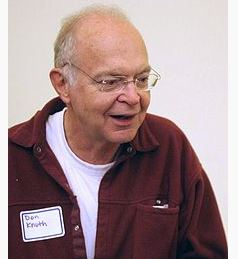
\includegraphics[width=3cm, height=3cm]{figuras/dona.JPG}
      \caption{Donald Ervin Knut, estadounidense experto en ciencias de la computación y matemático.}
      \label{f0} 
      \end{center}
\end{figure}

\subsection{\textbf{Definición}}
Es un método que permite encontrar, con el mínimo esfuerzo, una clave dada dentro de un conjunto de elementos. También se denomina método de "transformación de claves", "direccionamiento calculado","direccionamiento asociativo" o de "dispersión". En la técnica de Hashing se aplican cálculos o transformaciones aritméticas sobre la clave para producir directamente una dirección en una tabla o archivo de acceso directo.

\par De acuerdo a \citep{sierra}, define que los algoritmos hash son métodos de búsqueda, que proporcionan una longitud de búsqueda pequeña y una flexibilidad superior a la de otros métodos, como puede ser el método de búsqueda binaria que requiere que los elementos de la matriz
estén ordenados.

Según \citep{joyanes}, las tablas de dispersión o, simplemente, tablas hash son estructuras de datos que se usan en aplicaciones que manejan una secuencia de elementos. De tal forma que cada elemento tiene asociado un valor clave, que es un número entero positivo perteneciente a un rango de valores, relativamente pequeño. En estas organizaciones cada uno de los elementos ha de tener una clave que identifica de manera unívoca al elemento.

De acuerdo a \citep{weis}, Las tablas de hashing son una estructura de datos tipo diccionario que nos permite insertar, eliminar y buscar elementos a partir de una clave. Esta estructura se puede ver como un conjunto de entradas, donde cada una de ellas tiene asociada una clave única. Esto significa que una clave identifica unívocamente a una entrada en la tabla de hash.

\begin{figure}[H]
 \begin{center}
       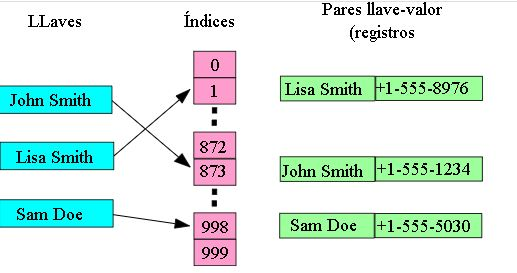
\includegraphics[width=8.5cm, height=5cm]{figuras/1.JPG}
      \caption{Ejemplo de Tabla Hash.}
      \label{f1} 
      \end{center}
\end{figure}
En la Figura ~\ref{f1}, se puede observar elementos de un Tabla Hash: llaves, índices y finalmente sus registros.

Según el Departamento de Lenguajes y Sistemas Informáticos de la Universidad de Alicante en España,\citep{organizacion} define al Método Hashing como \textbf{Ficheros de direccionamiento calculado (hashing)}, dado que la condición de búsqueda se realiza sobre un campo llamado \textit{direccionamiento calculado}.

Una función $h$ llamada función de direccionamiento calculado se aplica sobre el campo de direccionamiento calculado para obtener el bloque donde está el registro. Y los datos se almacenan de forma dispersa.

Por ejemplo: $h(K)$ = $K mod M$, donde:\\
$M$ : número de bloques a usar\\
$K$ : valor del campo de direccionamiento calculado. \\
Y se supone que $K$ es un valor de DNI = ‘21987239’, además el número total de bloques $M$=$20$ \\
$h(K)$ = $19$ (el registro se encuentra en el bloque número 19)

Y una vez conocido el número de bloque, un fichero de punteros apunta al bloque de disco, ver Figura ~\ref{Ualicante}.

\begin{figure}[H]
 \begin{center}
       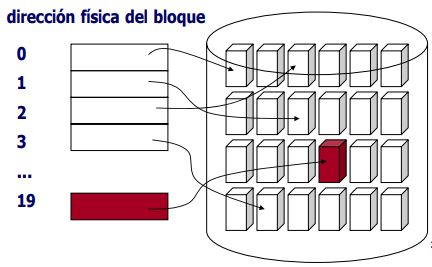
\includegraphics[width=7cm, height=2.7cm]{figuras/UAlicante.JPG}
      \caption{Dirección Física del bloque.}
      \label{Ualicante} 
      \end{center}
\end{figure}


%------------------------------------------------------------
\subsection{\textbf{Conceptos de Hashing}}
\begin{enumerate}[]
    \item {\textbf{Clave:}}
    \par Según \citep{carrillo}, la clave contiene el valor que permite ubicar mediante la función Hash la posición en el registro de ese elemento. Normalmente la clave es el campo que identifica en forma única la información. Por ejemplo: Documento de Identidad de una persona, Código de un empleado.
    \item {\textbf{Función Hash:}}
    \par De acuerdo a \citep{cairo}, una  función Hash se puede definir como una transformación de clave a una dirección. Al aplicar una función Hash a una clave se obtiene el número de cubeta en la cual se puede encontrar el registro con dicha clave. 
    \par Esta función consiste en asignar el índice a cada elemento mediante una transformación del elemento, el número obtenido es el índice del elemento.
    Hay diferentes funciones para transformar el elemento y son las siguientes:
    \begin{itemize}
        \item {\textbf{Método de la División o Aritmetica Modular}}
        \par Según \citep{wiki}, este método convierte la clave a un entero, se divide por el tamaño del rango del índice y toma el resto como resultado.
        
        Esta transformación implementada en lenguaje c++ quedaría de la siguiente manera:
        
        En la Figura ~\ref{divi}, se observa que la función $fhash$, representa al método de la división, que tiene un parámetro de tipo char \textbf{nom de longitud 20}, aquí recibe el array a calcular. Lo que realiza esta función dentro de su cuerpo es inicializar una variable suma en $0$ que almacenará el valor final de la suma de todas las letras del arreglo, basándose en el Código ASCII.
        
        \begin{figure}[H]
        \begin{center}
            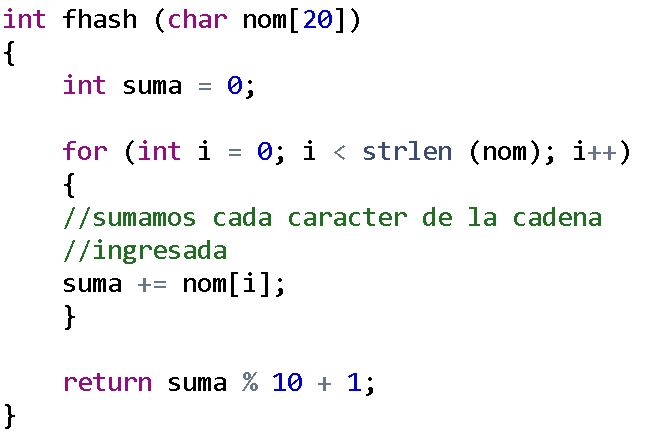
\includegraphics[width=6cm, height=3cm]{figuras/Divison.JPG}
            \caption{Implementación Método de la División.}
            \label{divi} 
        \end{center}
        \end{figure}

         El cual será recorrido con for hasta la longitud del array nom \textbf{(strlen(nom))}, finalmente retorna el resto de la suma con 10 + 1, obteniéndose así el valor de la clave.
        
        \item {\textbf{Mitad del cuadrado}}
        \par Según \citep{wiki}, consiste en elevar al cuadrado la clave y coger las cifras centrales. Este método también presenta problemas de colisión. En caso de que la cifra resultante tenga un número de dígitos impar, se toma el valor número y el anterior.
        
        Esta transformación implementada en lenguaje c++ quedaría de la siguiente manera:
        
        En la Figura ~\ref{mitad}, se observa que la función $fhash mitad cuadrado$, representa al método de mitad del cuadrado, que tiene un parámetro de tipo char \textbf{nom de longitud 20}, aquí recibe el array a calcular. Dentro del cuerpo de esta función, se inicializa la variables suma, cuadrado, contador y cifra. El for está encargado de recorrer todos los caracteres del array ingresado, e ir sumando acumulativamente en la variable suma, según Código ASCII. 
        
        Luego se obtiene el cuadrado de dicha variable, que se almacena en la variable cuadrado.
        Posteriormente, el primer while calcula la cantidad de dígitos de la variable cuadrado. Y el segundo while, separa todos los dígitos y los almacena en array tipo int de nombre numero.
        
        \begin{figure}[H]
        \begin{center}
            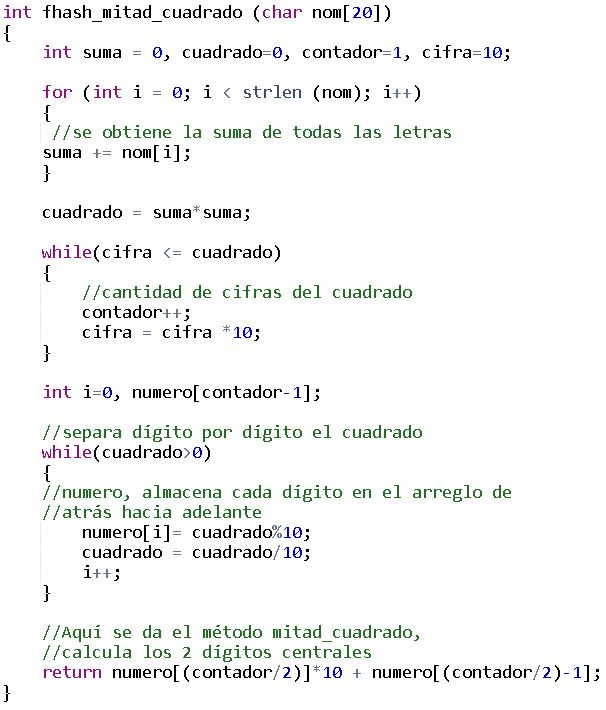
\includegraphics[width=7cm, height=9cm]{figuras/MitadCuadrado.JPG}
            \caption{Implementación Mitad del Cuadrado.}
            \label{mitad} 
        \end{center}
        \end{figure}
        
        Finalmente retorna los dos dígitos centrales del cuadrado.
        
        \item {\textbf{Truncamiento}}
        \par Según \citep{wiki}, consiste en ignorar parte del número y utilizar los elementos restantes como índice. También se produce colisión. Por ejemplo, si un número de 7 cifras se debe ordenar en un arreglo de elementos, se pueden tomar el segundo, el cuarto y el sexto para formar un nuevo número.
        
        Esta transformación implementada en lenguaje c++ quedaría de la siguiente manera:
        
        En la Figura ~\ref{trun}, se observa que la función $fhash truncamiento$, representa al método del truncamiento, que tiene un parámetro de tipo char \textbf{nom de longitud 20}, aquí recibe el array a calcular. Dentro del cuerpo de esta función, se inicializa la variables suma, cuadrado, contador y cifra. El for está encargado de recorrer todos los caracteres del array ingresado, e ir sumando acumulativamente en la variable suma, según Código ASCII.
        Aquí también se realiza como en el método anterior, para el primer while calcula la cantidad de dígitos de la variable cuadrado. 
        
        \begin{figure}[H]
        \begin{center}
            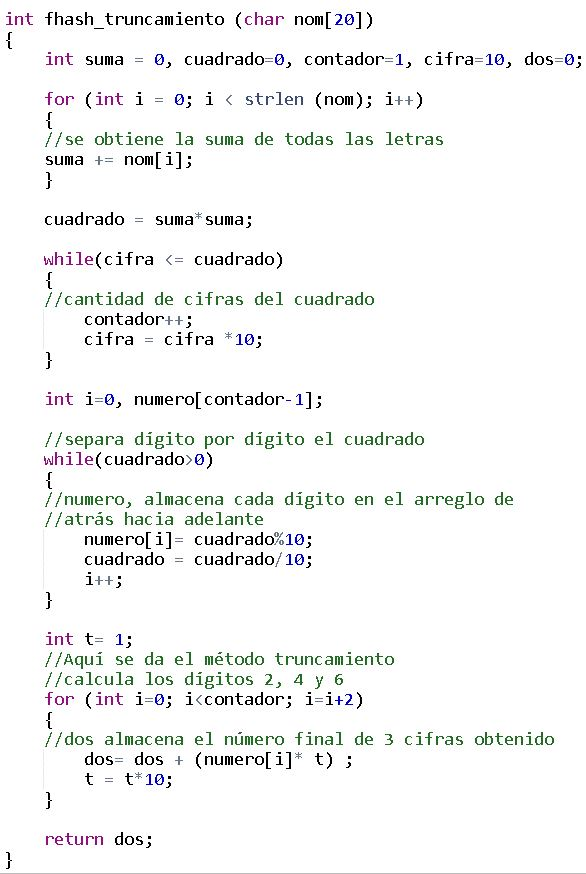
\includegraphics[width=7cm, height=9cm]{figuras/truncamiento.JPG}
            \caption{Implementación de Truncamiento.}
            \label{trun} 
        \end{center}
        \end{figure}
        
         Y el segundo while, separa todos los dígitos y los almacena en array tipo int de nombre numero.
        
        Adicionalmente, se agrega una estructura for que consiste en extraer los dígitos $2, 4$ y $6$, y dentro de la variable dos almacena el índice final que será posteriormente retornado.
        
        \item {\textbf{Plegamiento}}
        \par Según \citep{wiki}, consiste en dividir el número en diferentes partes, y operar con ellas (normalmente con suma o multiplicación). También se produce colisión. Por ejemplo, si dividimos el número de 7 cifras en 2, 2 y 3 cifras y se suman, dará otro número de tres cifras (y si no, se toman las tres últimas cifras).
        Esta transformación implementada en lenguaje c++ quedaría de la siguiente manera:
        
        En la Figura ~\ref{plega}, se se observa que la función $fhash plegamiento$, representa al método de la división, que tiene un parámetro de tipo char \textbf{nom de longitud 20}, aquí recibe el array a calcular.
        Dentro del cuerpo de esta función, se inicializa la variables suma, cuadrado, contador y cifra. El for está encargado de recorrer todos los caracteres del array ingresado, e ir sumando acumulativamente en la variable suma, según Código ASCII.
        
        \begin{figure}[H]
        \begin{center}
            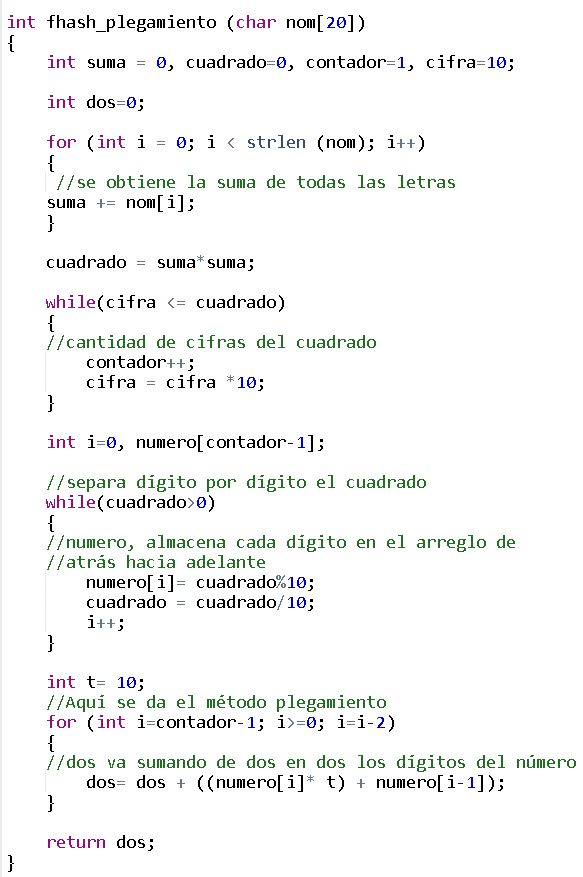
\includegraphics[width=7cm, height=8.5cm]{figuras/Plegamiento.JPG}
            \caption{Implementación de Plegamiento.}
            \label{plega} 
        \end{center}
        \end{figure}

        Aquí también se realiza como en los dos métodos anteriores, para el primer while calcula la cantidad de dígitos de la variable cuadrado. Y el segundo while, separa todos los dígitos y los almacena en array tipo int de nombre numero.
        
        Asimismo, se agrega una estructura for que consiste en extraer de dos en dos los dígitos, en ir realizando sumas acumulativas y dentro de la variable dos almacena el índice final que como termino de la función es retornado.
        
    \end{itemize}
\end{enumerate}

%---------------------------------------------------------------------------
\section{\textbf{Implementación de las Funciones para el Método Disperso o Hash en C++}} 
Para la implementación de este método hemos considerado realizar un registro de datos personales de una persona, así que los siguientes códigos se basan en ello. 
\begin{enumerate}[]
    \item {\textbf{Estructura Encabezado:}}
        \par Para definir el encabezado, ver Figura ~\ref{f-enca}, se usó \textbf{struct} para poder almacenar varios campos, en este caso \textbf{NRS} que es la variable que almacena el número total de registros y \textbf{URE} que es la variable que almacena el último registro eliminado, además de los punteros \textbf{ed} y \textbf{ec} para el archivo dispersión y archivo colisión respectivamente.
        \begin{figure}[H]
            \begin{center}
            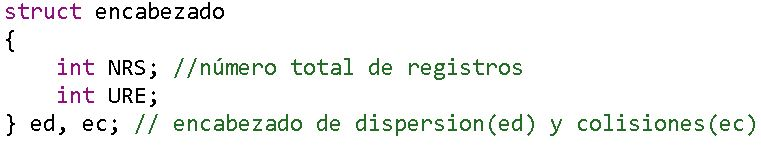
\includegraphics[width=8cm, height=1.8cm]{figuras/encabezado.JPG}
            \caption{Código de Estructura Encabezado.}
            \label{f-enca} 
            \end{center}
        \end{figure}
    \item {\textbf{Estructura Registro:}}
        \par Para definir el registro, obsérvese en la Figura ~\ref{f-reg}, se usó \textbf{struct} para poder almacenar varios campos, en este caso los datos personales de una persona y usamos: \textbf{NR} que es la variable que almacena el número de registro, el campo \textbf{dni} que es la variable que almacena el número de dni de una persona, el campo \textbf{nombre} que es la variable que almacena el nombre, el campo \textbf{apellido} que es la variable que almacena el apellido, el campo \textbf{email} que es la variable que almacena el correo electrónico, el campo \textbf{celular} que es la variable que almacena el número de celular, el campo \textbf{SR} que es la variable que almacena el siguiente registro, el campo \textbf{ARE} que es la variable que almacena el anterior registro eliminado y además de los punteros \textbf{r} y \textbf{s} para el archivo dispersión y archivo colisión respectivamente.
         \begin{figure}[H]
            \begin{center}
            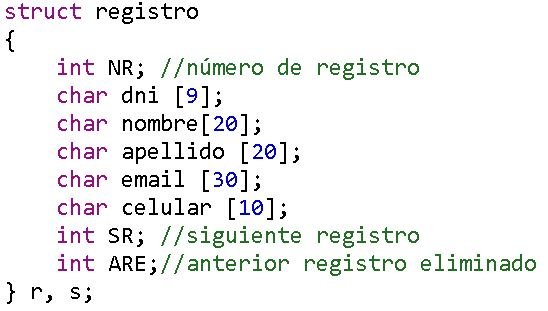
\includegraphics[width=6cm, height=3cm]{figuras/registro.JPG}
            \caption{Código de Estructura Encabezado.}
            \label{f-reg} 
            \end{center}
        \end{figure}
    \item {\textbf{Escribir:}}
        \par En la función escribir, obsérvese la primera parte en la Figura ~\ref{f-escribir1}, inicialmente se abren ambos archivos, el archivo dispersión y archivo colisión, es decir para ser escritos; además se inicializan las variables ed y ec en sus campo NRS, que representa numero total de registros existentes en los archivos; y actualiza escribiendo en el encabezado. 
        
        Dentro de un do while, se solicita ingresar al usuario la información de los campos para cada registro. Luego actualiza el campo SR con -1, que representa que no hay siguiente. También calcula el valor para el campo NR, obteniendo con la función fhash y enviándole como parámetro, el campo nombre ingresado anteriormente.
        
        Para el condicional, evalúa si no hay colisión, graba de forma dispersa, basándose en el índice hash, en el archivo $*.txt$. Aquí también se actualiza de la variable ed el campo NRS, incrementándose en 1; posiciona y escribe en el registro.
        
        %\vspace{-20 mm}
        \begin{figure}[H]
            \begin{center}
            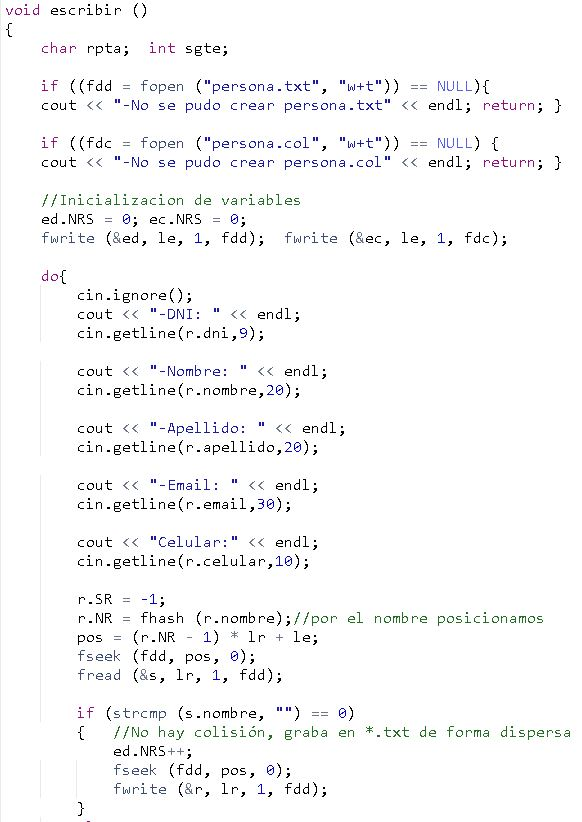
\includegraphics[width=9cm, height=10cm]{figuras/escribir 1.JPG}
            \caption{Código de Función Escribir - Parte 1.}
            \label{f-escribir1} 
            \end{center}
        \end{figure}
        
        En la segunda parte de esta función, obsérvese Figura ~\ref{f-escribir2}, se encuentra el else del if anterior, aquí se considera cuando si existe colisión, por lo que se escribe o graba en el archivo $*.col$, de forma secuencial. Actualizando de igual manera el campo NRS de la variable ec, que pertenece a este archivo.
        
        \begin{figure}[H]
            \begin{center}
            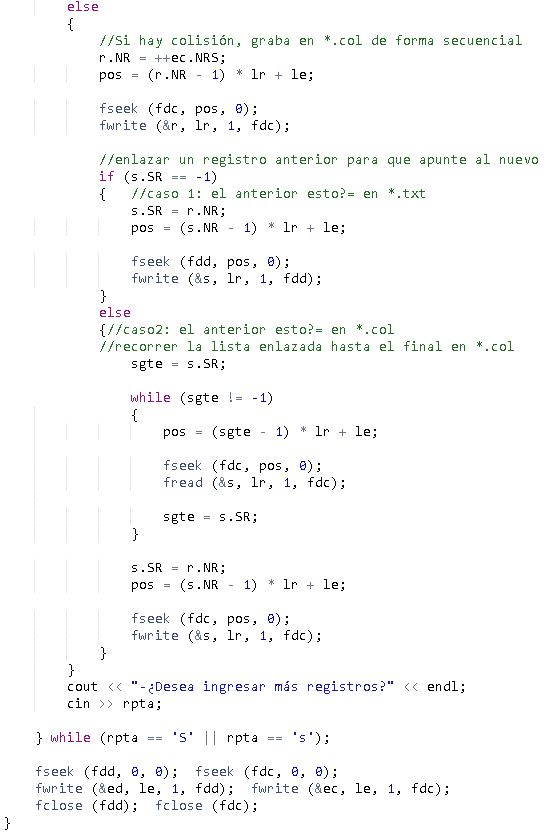
\includegraphics[width=8cm, height=15cm]{figuras/escribir2.JPG}
            \caption{Código de Función Escribir - Parte 2.}
            \label{f-escribir2} 
            \end{center}
        \end{figure}
        
         Luego con un if else, se enlaza un registro anterior para que apunte al nuevo. Evalúa de cumplirse la igualdad entre -1 y el campo SR de s, para el caso 1, si el anterior estará en  $*.txt$, de ser cierto ingresa y actualiza el campo SR, posiciona y escribe. Para el caso 2, el anterior esta en $*.col$, por lo que actualiza el sgte y con un while recorre la lista enlazada hasta el final, aquí también se posiciona y escribe.
        Para el do while mencionado inicialmente, se dará si rpta es S o s, de no cumplirse se termina. Finalmente se actualiza los encabezados y cierra de los dos archivos.
        
    \item {\textbf{Mostrar:}}
        \par Para definir la función mostrar, ver Figura ~\ref{f-mos}, primero, abrimos ambos archivos, es decir, el archivo dispersión y archivo colisión respectivamente, luego, se lee el encabezado para mostrar datos convenientemente, también a través de \textbf{fread} se lee los datos a mostrar en pantalla y se hace lo mismo con el archivo colisión, finalmente cerramos ambos archivos.
         \begin{figure}[H]
            \begin{center}
            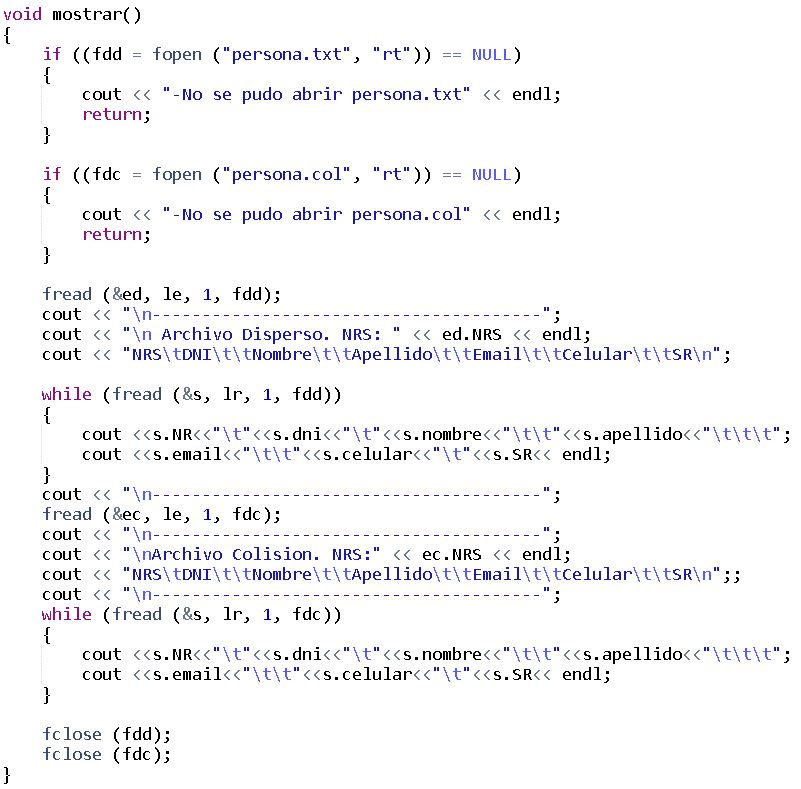
\includegraphics[width=9cm, height=9cm]{figuras/mostrar.JPG}
            \caption{Código de Función Mostrar.}
            \label{f-mos} 
            \end{center}
        \end{figure}
    \item {\textbf{Buscar:}}
        \par En la función buscar, obsérvese en la Figura ~\ref{f-bus}, inicialmente se abren ambos archivos, el archivo dispersión y archivo colisión respectivamente, es decir para que puedan ser leídos y escritos; luego solicita digitar al usuario el nombre que desea buscar. Después, se calcula con la función $fhash$, el índice, calcula pos y lee.
        
        Para la \textbf{búsqueda en el archivo dispersión}, se realiza dos condicionales, el primer if evalua si existe registro con ese hash, de no ser cierto retorna con un mensaje. Y en el segundo if realiza las comparaciones con cada registro del archivo, cuando lo encuentra, muestra la información de sus campos y retorna. De no cumplirse ninguno de los dos if muestra que no existe en el archivo.
        
        Por otro lado, para la \textbf{búsqueda en el archivo de colisión}, se inicializa la variable $sgte$ con el campo SR de s, y través del while como primer paso, se evalua que mientras sea diferente de -1 y va actualizando el sgte, entrará a calcular pos, posiciona y leer; con \textbf{fseek y fread}. Con un condicional, realiza las comparaciones con cada nombre del registro, si coincide con uno entonces muestra la información de sus campos y retorna. De no cumplirse en el if y no encontrarse el nombre, muestra un mensaje que no existe en el archivo.
        %\vspace{-5 mm}
        \begin{figure}[H]
            \begin{center}
            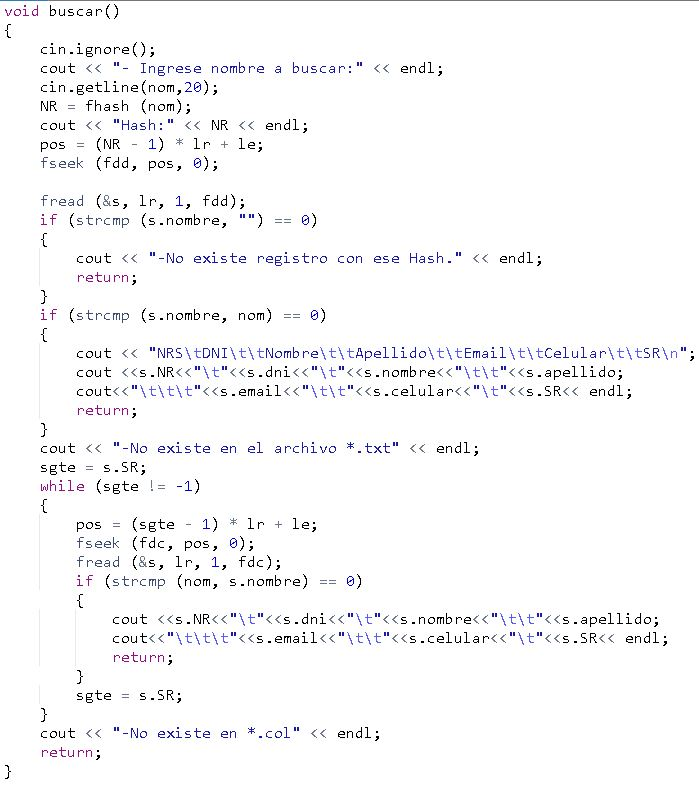
\includegraphics[width=8.5cm, height=10cm]{figuras/buscar.JPG}
            \caption{Código de Función Buscar.}
            \label{f-bus} 
            \end{center}
        \end{figure}
    \item {\textbf{Insertar:}}
        \par En esta función, ver Figura ~\ref{f-inser}, es de manera similar que la función escribir, solo que aquí se \textbf{evita la inicialización del campo NRS} en las variables ed y ec; porque esos son campos globales y puede existir la posibilidad que ya existan registros, por lo que si las inicializamos nuestro programa no funcionará y no almacenara los registros de manera adecuada, debido a que en ese campo se inicializa en 0. 
        
        Luego todo es exactamente igual que la función escribir.
         \begin{figure}[H]
            \begin{center}
            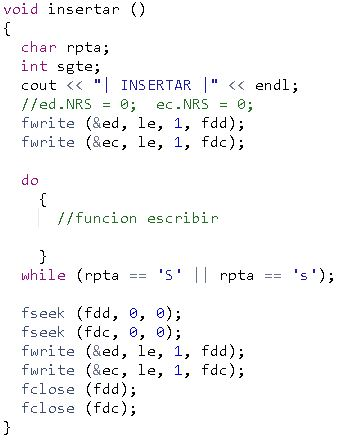
\includegraphics[width=6cm, height=6cm]{figuras/insertar.JPG}
            \caption{Código de Función Insertar.}
            \label{f-inser} 
            \end{center}
        \end{figure}
    
    \item {\textbf{Modificar:}}
        \par En la función modificar, ver Figura ~\ref{f-modifi}, inicialmente se abre el archivo para ser modificado $r + t$, es decir para poder leer y escribir, \textbf{persona.txt}, luego con \textbf{fread}, se lee el encabezado y se solicita digitar al usuario el nombre que desea modificar.
        
        Después, a través del while como primer paso, se \textbf{busca en los registros} realizándose comparaciones, de encontrarse, se realiza el segundo paso donde \textbf{solicita digitar el nuevo Email}, actualizando dicha información a través de posicionar y escribir, con \textbf{fseek y fwrite} en el registro, por otro lado, de no encontrarse el nombre muestra un mensaje. Finalmente actualiza el encabezado, y cierra el archivo.
        
        \begin{figure}[H]
            \begin{center}
            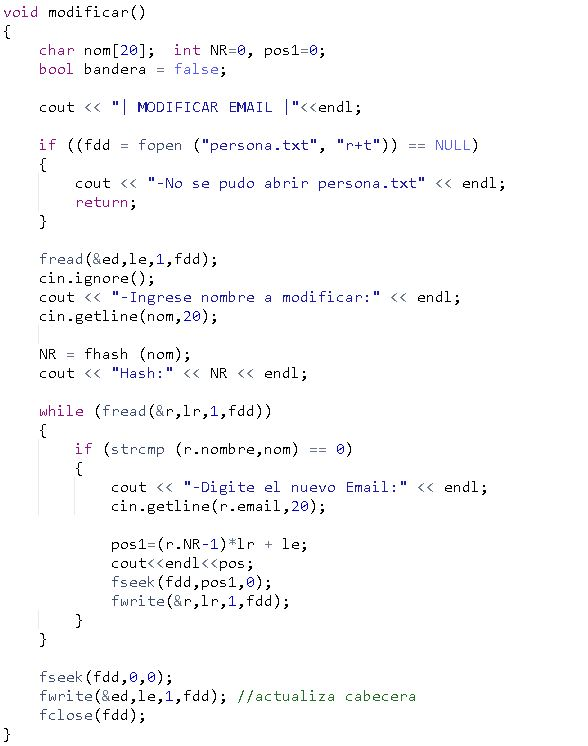
\includegraphics[width=8.5cm, height=10cm]{figuras/modificar.JPG}
            \caption{Código de Función Modificar.}
            \label{f-modifi} 
            \end{center}
        \end{figure}
        
    \item {\textbf{Eliminar:}}
        \begin{figure}[H]
            \begin{center}
            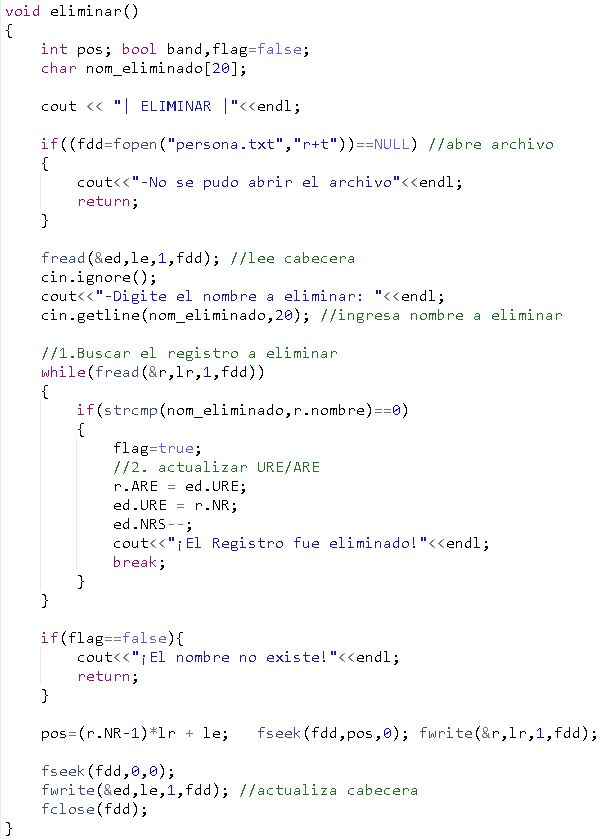
\includegraphics[width=8.5cm, height=10cm]{figuras/eliminado.JPG}
            \caption{Código de Función Eliminar.}
            \label{f-elimi} 
            \end{center}
        \end{figure}
        
        \par Para la función eliminar, obsérvese en la Figura ~\ref{f-elimi}, inicialmente se abre el archivo \textbf{persona.txt}, luego con fread, se lee el encabezado y se solicita digitar al usuario el nombre que desea eliminar.
        
        Después, a través del while como primer paso, se \textbf{busca en los registros} realizándose comparaciones, de encontrarse, se realiza el segundo paso donde \textbf{actualiza los valores URE/ARE}, asignándole a URE, NR, que es el índice hash, el URE, representa cuál es último elemento eliminado y al campo ARE, -1, que representa que está eliminado; por otro lado, de no encontrarse el nombre muestra un mensaje. Finalmente posiciona y escribe con \textbf{fseek y fwrite} tanto en el registro y actualiza el encabezado, y cierra el archivo.
        
\end{enumerate}

\section{\textbf{Conclusión}}
Este informe presentó información relevante acerca del Método Disperso o Hash, se ha explicado los conceptos teóricos relacionados con este, cabe precisar que si el valor hash obtenido de los caracteres de la información original sobre la que se aplica los algoritmos o métodos hash, varía cualquier de sus caracteres, varía el valor final. Además de permitir conocer sobre la implementaciones de los métodos hash, con sus respectivas explicaciones, además de otras funciones que permiten la creación de dos registros, con extensiones, uno $*.txt$. y otro $*.col$. en los que se puede escribir, mostrar, buscar, modificar y eliminar registros. 

%-------------------------------------------------------
\medskip
\bibliography{refer}
\end{document}
